% =====================================================================
% Relatório da Avaliação M3 - Servidor Aperiódico (template IEEE, A4)
% Compilação: pdflatex Relatorio_STR_M3.tex (duas vezes)
% Os gráficos (pgfplots) leem os arquivos da pasta dados/, que deve
% ficar ao lado deste .tex.
% =====================================================================
\documentclass[conference,a4paper]{IEEEtran}
\usepackage[utf8]{inputenc}
\usepackage[T1]{fontenc}
\usepackage{amsmath,amssymb}
\usepackage{booktabs,array,multirow}
\usepackage{graphicx,microtype}
\usepackage{tikz}
\usetikzlibrary{arrows.meta,positioning,shapes.geometric}
\usepackage{pgfplots}
\usepgfplotslibrary{groupplots}
\pgfplotsset{compat=1.16}
\usepackage{listings}
\usepackage[hidelinks]{hyperref}

% Cores dos dois modos de carga (usadas em todos os gráficos)
\definecolor{azul}{HTML}{2A78D6}     % nanosleep
\definecolor{laranja}{HTML}{EB6834}  % NOP
\definecolor{cinza}{HTML}{6B6B6B}

\lstset{language=C,basicstyle=\ttfamily\fontsize{6.5}{7.6}\selectfont,
  breaklines=true,frame=single,xleftmargin=2pt,xrightmargin=2pt,
  columns=fullflexible,keepspaces=true,showstringspaces=false,
  commentstyle=\itshape\color{cinza},aboveskip=6pt,belowskip=2pt,
  captionpos=b}

\renewcommand{\abstractname}{Resumo}
\renewcommand{\IEEEkeywordsname}{Palavras-chave}
\renewcommand{\tablename}{Tabela}
\renewcommand{\figurename}{Figura}
\renewcommand{\lstlistingname}{Trecho}
\hyphenation{NAV-PLAN}

\begin{document}

\title{Servidor periódico para atendimento de requisições aperiódicas: aplicação à tarefa NAV\_PLAN}

\author{\IEEEauthorblockN{Thiago Fernandes Jacques}
\IEEEauthorblockA{Engenharia de Computação --- Universidade do Vale do Itajaí (UNIVALI)\\
Sistemas em Tempo Real --- Avaliação M3 --- Professor: Felipe Viel}}

\maketitle

% ---------------------------------------------------------------------
\begin{abstract}
Este trabalho implementa em C, com \emph{pthreads} e escalonamento SCHED\_FIFO, um servidor periódico que atende requisições aperiódicas em conjunto com quatro tarefas periódicas. A função aperiódica escolhida é a NAV\_PLAN do autopiloto da M2, que trata eventos de navegação (NAV) e de telemetria (TEL). O servidor tem período $T_s=50$ ms e orçamento $C_s=20$ ms. Cada requisição registra os instantes de chegada, início e fim, dos quais se obtêm a espera na fila, o tempo de execução e o tempo de resposta. A carga foi simulada de dois modos: com \texttt{nanosleep}, em que a thread dorme, e com um laço de NOP, em que ela ocupa o processador. Em duas execuções de 10 s, fixadas em um núcleo, a espera nunca ultrapassou o período do servidor (máximo de 49,79 ms) e o maior tempo de resposta foi 53,44 ms, de acordo com o limite $T_s+C$. O laço de NOP reproduziu o tempo nominal de execução (3,50 ms), enquanto o \texttt{nanosleep} acrescentou cerca de 0,19 ms, sem efeito relevante na resposta.
\end{abstract}

\begin{IEEEkeywords}
Tempo real, servidor periódico, tarefas aperiódicas, SCHED\_FIFO, tempo de resposta.
\end{IEEEkeywords}

% ---------------------------------------------------------------------
\section{Introdução}
Sistemas de tempo real combinam tarefas periódicas, com ativação regular e prazo conhecido, e eventos aperiódicos, cuja chegada não é previsível. Se os eventos aperiódicos forem atendidos sem controle, podem ocupar o processador e fazer as tarefas periódicas perderem prazos. O servidor periódico resolve esse problema: é uma tarefa com período $T_s$ e orçamento $C_s$ que, a cada período, atende os pedidos pendentes até esgotar o orçamento ou a fila. Assim, o uso do processador pelos aperiódicos fica limitado a $C_s/T_s$.

Este trabalho aplica o servidor à tarefa NAV\_PLAN, que na M2 era disparada por sensores touch. Aqui os eventos são gerados por software, o que torna o experimento repetível. O objetivo é implementar o servidor, medir a espera, a execução e a resposta de cada requisição e verificar se os resultados seguem o comportamento esperado do modelo.

% ---------------------------------------------------------------------
\section{Enunciado do projeto}
A Avaliação M3 pede que se evolua o trabalho da M2 e se faça a análise temporal de um servidor aperiódico. As tarefas periódicas e esporádicas (T1 a T4) são escalonadas diretamente pelo processador, e as aperiódicas vão para uma fila de serviço. O servidor, ele próprio uma tarefa periódica, acorda a cada $T_s$ com um orçamento $C_s$, consome a fila enquanto houver orçamento e volta a dormir até o próximo período.

Os requisitos são: escolher uma função aperiódica da M2 e reproduzi-la com \emph{pthreads} usando o servidor de exemplo fornecido; programar em C ou C++; usar prioridade de tempo real (SCHED\_FIFO); manter a fila com \texttt{enqueue\_job} e \texttt{dequeue\_job}; tornar o servidor periódico com \texttt{clock\_nanosleep} em tempo absoluto; comentar o código; e executar com privilégio de superusuário. A função escolhida foi a NAV\_PLAN, que na M2 tinha prioridade 3 e prazo de 20 ms.

% ---------------------------------------------------------------------
\section{Técnicas utilizadas}

\subsection{Arquitetura}
A Fig.~\ref{fig:arq} mostra a organização, que segue o modelo do enunciado. O gerador coloca as requisições na fila de serviço; o servidor as retira e as executa. O servidor e as tarefas periódicas disputam o processador, escalonado pelo Linux com SCHED\_FIFO, em que a thread pronta de maior prioridade sempre executa. A Tabela~\ref{tab:param} resume os parâmetros. A utilização total reservada é de 66\%: 40\% do servidor ($C_s/T_s$) e cerca de 26\% das tarefas periódicas.

\begin{figure}[!t]
\centering
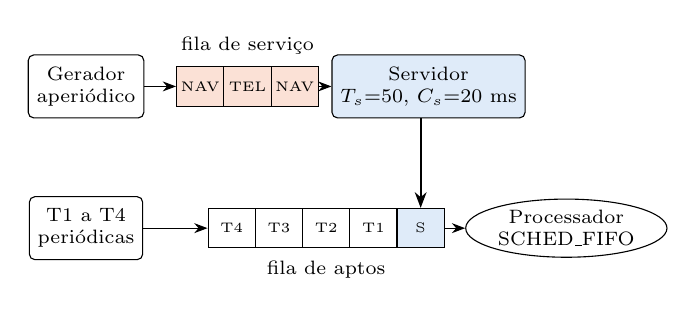
\begin{tikzpicture}[>=Stealth, font=\scriptsize,
  caixa/.style={draw, rounded corners=2pt, align=center, minimum height=8mm, inner xsep=3pt},
  cel/.style={draw, minimum width=6mm, minimum height=5mm, inner sep=0pt, font=\tiny}]
% linha superior: requisicoes aperiodicas
\node[caixa] (gen) at (-3.35,0) {Gerador\\aperiódico};
\node[cel, fill=laranja!20] (a1) at (-1.9,0) {NAV};
\node[cel, fill=laranja!20] (a2) at (-1.3,0) {TEL};
\node[cel, fill=laranja!20] (a3) at (-0.7,0) {NAV};
\node[above=1pt of a2] {fila de serviço};
\node[caixa, fill=azul!15] (srv) at (1.0,0) {Servidor\\$T_s{=}50$, $C_s{=}20$ ms};
\draw[->] (gen) -- (a1);
\draw[->] (a3) -- (srv);
% linha inferior: fila de aptos
\node[caixa] (per) at (-3.35,-1.8) {T1 a T4\\periódicas};
\node[cel] (p4) at (-1.5,-1.8) {T4};
\node[cel] (p3) at (-0.9,-1.8) {T3};
\node[cel] (p2) at (-0.3,-1.8) {T2};
\node[cel] (p1) at ( 0.3,-1.8) {T1};
\node[cel, fill=azul!15] (ps) at (0.9,-1.8) {S};
\node[below=1pt of p2] {fila de aptos};
\node[ellipse, draw, align=center, inner sep=1pt] (cpu) at (2.75,-1.8) {Processador\\SCHED\_FIFO};
\draw[->] (per) -- (p4);
\draw[->] (ps) -- (cpu);
\draw[->, semithick] (srv.south -| ps) -- (ps.north);
\end{tikzpicture}
\caption{Arquitetura do sistema. As requisições aperiódicas passam pela fila de serviço e são executadas pelo servidor (S), que disputa o processador com T1 a T4.}
\label{fig:arq}
\end{figure}

\begin{table}[!t]
\centering
\caption{Parâmetros das tarefas no experimento}
\label{tab:param}
\footnotesize
\setlength{\tabcolsep}{4pt}
\begin{tabular}{lrrrr}
\toprule
Tarefa & Período (ms) & Carga (ms) & Prioridade & Utilização \\
\midrule
Servidor & 50 & 20 (orçamento) & 60 & 40,0\% \\
T1 & 40 & 5 & 50 & 12,5\% \\
T2 & 80 & 5 & 50 & 6,3\% \\
T3 & 120 & 5 & 50 & 4,2\% \\
T4 & 160 & 5 & 50 & 3,1\% \\
Gerador & 30 a 120 & --- & comum & --- \\
\midrule
\multicolumn{5}{l}{NAV\_PLAN (executada pelo servidor): NAV 3,5 ms; TEL 0,5 ms} \\
\bottomrule
\end{tabular}
\end{table}

\subsection{Fila de requisições}
A fila é uma lista ligada protegida por mutex (Trecho~\ref{lst:fila}). Cada nó guarda um ponteiro para a função a executar e um ponteiro genérico para seu argumento. Como o servidor só conhece esse par, o mesmo mecanismo serve para qualquer tipo de job.

\begin{lstlisting}[caption={Fila de jobs, do código de exemplo.},label={lst:fila}]
typedef void (*job_func_t)(void *arg);
typedef struct job {
    job_func_t func;   // funcao a executar
    void *arg;         // argumento da funcao
    struct job *next;
} job_t;

void enqueue_job(job_func_t f, void *arg) {
    job_t *j = malloc(sizeof(job_t));
    j->func = f;  j->arg = arg;  j->next = NULL;
    pthread_mutex_lock(&queue_mutex);
    if (queue_tail) queue_tail->next = j;
    else            queue_head = j;
    queue_tail = j;
    pthread_mutex_unlock(&queue_mutex);
}
\end{lstlisting}

\subsection{Job NAV\_PLAN}
O gerador cria uma estrutura \texttt{nav\_req\_t} com o tipo do evento e o instante de chegada, e a enfileira junto com a função \texttt{nav\_plan\_job} (Trecho~\ref{lst:job}). O servidor repassa o ponteiro ao job, que lê os campos, simula o trabalho e libera a memória. O evento NAV simula o cálculo de rota por 3,5 ms; o TEL imprime a atitude e simula 0,5 ms.

\begin{lstlisting}[caption={Argumento, job NAV\_PLAN e geração do pedido.},label={lst:job}]
typedef enum { EV_NAV = 0, EV_TEL = 1 } evt_t;
typedef struct {
    evt_t ev;            // tipo do evento
    int64_t chegada_us;  // instante de chegada
} nav_req_t;

void nav_plan_job(void *arg) {
    nav_req_t *req = (nav_req_t *)arg;
    int64_t task_start_us = now_us();
    if (req->ev == EV_NAV) busy_us(3500);   // rota
    else                   busy_us(500);    // telemetria
    int64_t task_end_us = now_us();
    // calcula e imprime exec, espera e resposta
    free(arg);
}

// no gerador: cria o pedido e carimba a chegada
nav_req_t *p = malloc(sizeof(nav_req_t));
p->ev = (counter++ % 2 == 0) ? EV_NAV : EV_TEL;
p->chegada_us = now_us();
enqueue_job(nav_plan_job, p);
\end{lstlisting}

\subsection{Modos de simulação de carga}\label{sec:modos}
O código de exemplo simula o trabalho com \texttt{nanosleep}: a thread dorme e não usa o processador. Para comparar, a função \texttt{busy\_us} ganhou um segundo modo, ativado com \texttt{./servidor\_aperiodico nop}, em que a thread executa um laço de NOP até o tempo acabar e ocupa o processador durante todo o intervalo (Trecho~\ref{lst:carga}). O modo vale para o job e para T1 a T4.

\begin{lstlisting}[caption={Simulação de carga nos dois modos.},label={lst:carga}]
static void busy_us(long us) {
    if (g_modo_nop) {                      // ocupa a CPU
        int64_t inicio = now_us();
        while ((now_us() - inicio) < us)
            __asm__ __volatile__("nop");
    } else {                               // dorme
        struct timespec req = {0};
        req.tv_nsec = us * 1000L;
        nanosleep(&req, NULL);
    }
}
\end{lstlisting}

\subsection{Servidor periódico}
A cada período, o servidor retira jobs da fila e os executa enquanto o tempo decorrido no período for menor que $C_s$ (Trecho~\ref{lst:servidor}). Quando a fila esvazia ou o orçamento acaba, ele dorme até a próxima liberação, calculada em tempo absoluto com \texttt{clock\_nanosleep}, o que evita o acúmulo de atraso. O orçamento é verificado depois de cada job, então um job iniciado perto do limite pode ultrapassá-lo em até um tempo de execução (no máximo cerca de 4 ms).

\begin{lstlisting}[caption={Laço principal do servidor.},label={lst:servidor}]
while (1) {
    timespec_add_ns(&next_release, Ts);
    clock_gettime(CLOCK_MONOTONIC, &start_period);
    long elapsed = 0;
    while (elapsed < Cs) {
        pthread_mutex_lock(&queue_mutex);
        job_t *j = dequeue_job();
        pthread_mutex_unlock(&queue_mutex);
        if (!j) break;                   // fila vazia
        j->func(j->arg);                 // executa o job
        clock_gettime(CLOCK_MONOTONIC, &t_after);
        elapsed = timespec_diff_ns(&t_after, &start_period);
        free(j);
    }
    clock_nanosleep(CLOCK_MONOTONIC, TIMER_ABSTIME,
                    &next_release, NULL);
}
\end{lstlisting}

\subsection{Métricas}
Com os instantes de chegada $t_c$, início $t_i$ e fim $t_f$, lidos de \texttt{CLOCK\_MONOTONIC}, cada requisição registra
\begin{equation}
C=t_f-t_i,\qquad W=t_i-t_c,\qquad R=t_f-t_c=W+C,
\end{equation}
isto é, tempo de execução, espera na fila e tempo de resposta. A Fig.~\ref{fig:tempo} ilustra as três grandezas. O job acumula, em variáveis globais por tipo de evento, a quantidade, a soma, o mínimo e o máximo de cada métrica, e o \texttt{main} imprime o resumo ao fim da execução.

\begin{figure}[!t]
\centering
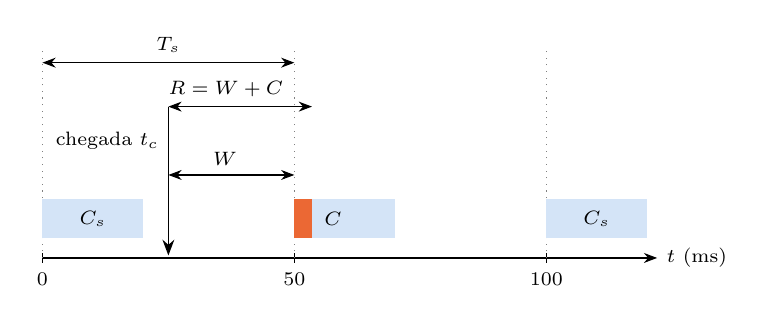
\begin{tikzpicture}[x=0.064cm, y=0.62cm, >=Stealth, font=\scriptsize]
\draw[->] (0,0) -- (122,0) node[right] {$t$ (ms)};
\foreach \x in {0,50,100} {
  \draw (\x,0.1) -- (\x,-0.1) node[below] {\x};
  \draw[dotted, gray] (\x,0) -- (\x,4.3);
  \fill[azul!20] (\x,0.4) rectangle (\x+20,1.2);
}
\node at (10,0.8) {$C_s$};
\node at (110,0.8) {$C_s$};
\fill[laranja] (50,0.4) rectangle (53.5,1.2);
\node[right] at (54,0.8) {$C$};
\draw[->, semithick] (25,3.1) -- (25,0.05);
\node[left] at (25,2.4) {chegada $t_c$};
\draw[<->] (25,1.7) -- (50,1.7) node[pos=0.45, above] {$W$};
\draw[<->] (25,3.1) -- (53.5,3.1) node[pos=0.4, above] {$R=W+C$};
\draw[<->] (0,4.0) -- (50,4.0) node[midway, above] {$T_s$};
\end{tikzpicture}
\caption{Atendimento de uma requisição. Ela chega em $t_c$, espera ($W$) até o servidor acordar em 50 ms e é executada ($C$, em laranja) dentro do orçamento $C_s$ (em azul). A espera nunca passa de $T_s$, logo $R\le T_s+C$.}
\label{fig:tempo}
\end{figure}

% ---------------------------------------------------------------------
\section{Metodologia de teste}
O programa foi compilado com \texttt{gcc -O2 -Wall} e executado com \texttt{sudo}, necessário para SCHED\_FIFO, fixado em um único núcleo com \texttt{taskset -c 0}. Fixar o núcleo obriga todas as threads a disputar o mesmo processador; sem isso, elas rodariam em paralelo e a interferência não apareceria. Cada modo de carga foi executado uma vez, por 10 s, e a saída foi gravada em arquivo (Trecho~\ref{lst:saida}). Os gráficos foram gerados a partir desses arquivos.

\begin{lstlisting}[basicstyle=\ttfamily\fontsize{6}{7}\selectfont,caption={Comandos de execução e trecho da saída do modo NOP, com o resumo impresso pelo programa.},label={lst:saida}]
gcc -O2 -Wall servidor_aperiodico.c -o servidor_aperiodico -pthread
sudo taskset -c 0 ./servidor_aperiodico     | tee saida_sleep.log
sudo taskset -c 0 ./servidor_aperiodico nop | tee saida_nop.log

Modo de carga: NOP (ocupa a CPU)
[T1] executando
NAV_PLAN: Evento NAV recebido
NAV_PLAN: chegada=9340044.68ms inicio=9340089.85ms fim=9340093.36ms
          exec=3.50ms espera=45.17ms resposta=48.67ms
...
===== RESUMO (ms) =====
NAV: 66 requisicoes
  exec     min=3.50  media=3.50  max=3.53
  espera   min=2.30  media=27.57  max=49.79
  resposta min=5.80  media=31.07  max=53.30
TEL: 65 requisicoes
  exec     min=0.50  media=0.51  max=0.54
  espera   min=1.87  media=25.45  max=47.82
  resposta min=2.41  media=25.96  max=48.33
\end{lstlisting}

% ---------------------------------------------------------------------
\section{Resultados}

A Tabela~\ref{tab:result} reúne as métricas das duas execuções: 136 requisições no modo \texttt{nanosleep} e 131 no modo NOP, divididas igualmente entre NAV e TEL.

\begin{table}[!t]
\centering
\caption{Resultados por modo de carga e tipo de evento (tempos em ms)}
\label{tab:result}
\footnotesize
\setlength{\tabcolsep}{5pt}
\begin{tabular}{lrrrr}
\toprule
 & \multicolumn{2}{c}{\texttt{nanosleep}} & \multicolumn{2}{c}{NOP} \\
\cmidrule(lr){2-3}\cmidrule(lr){4-5}
Métrica & NAV & TEL & NAV & TEL \\
\midrule
Requisições            & 68    & 68    & 66    & 65    \\
\midrule
Execução média $\bar C$ & 3,69  & 0,56  & 3,50  & 0,51  \\
Execução máx. $C_{\max}$ & 3,90 & 0,66  & 3,53  & 0,54  \\
\midrule
Espera média $\bar W$   & 26,59 & 25,79 & 27,57 & 25,45 \\
Espera máx. $W_{\max}$  & 49,54 & 49,63 & 49,79 & 47,82 \\
\midrule
Resposta média $\bar R$ & 30,28 & 26,34 & 31,07 & 25,96 \\
Resposta máx. $R_{\max}$ & 53,44 & 50,18 & 53,30 & 48,33 \\
Respostas $\le 20$ ms  & 29\%  & 35\%  & 29\%  & 35\%  \\
Respostas $> 50$ ms    & 4     & 1     & 5     & 0     \\
\bottomrule
\end{tabular}
\end{table}

\subsection{Tempo de execução}
Com \texttt{nanosleep}, a execução média ficou 0,19 ms acima do nominal no NAV (3,69 ms) e 0,06 ms acima no TEL (0,56 ms). Esse acréscimo é o tempo que o sistema leva para acordar a thread depois do \texttt{nanosleep}, somado ao custo das impressões. Com o laço de NOP, a execução coincidiu com o nominal (3,50 e 0,51 ms) e quase não variou (máximo de 3,53 ms), pois o laço confere o relógio continuamente e não depende do escalonador para voltar a executar. Mesmo com T1 a T4 ocupando o processador no modo NOP, nenhum job foi interrompido, já que o servidor tem a maior prioridade.

\subsection{Espera na fila}
Nos dois modos, a espera ficou sempre abaixo de 50 ms ($T_s$), com média próxima de 26 ms, metade do período. A Fig.~\ref{fig:hist} mostra por quê: as esperas se espalham por todo o intervalo de 0 a 50 ms, perto da contagem esperada para uma distribuição uniforme (linha tracejada). Isso ocorre porque o gerador sorteia os instantes de chegada, que caem em pontos aleatórios do período do servidor.

\begin{figure}[!t]
\centering
\begin{tikzpicture}
\begin{groupplot}[
  group style={group size=1 by 2, vertical sep=0.9cm,
               xlabels at=edge bottom, xticklabels at=edge bottom},
  width=\columnwidth, height=3.6cm,
  xmin=0, xmax=50, ymin=0, ymax=25,
  xtick={0,10,20,30,40,50}, ytick={0,10,20},
  ymajorgrids, grid style={gray!25},
  tick label style={font=\scriptsize}, label style={font=\footnotesize},
  ylabel={Requisições}]
\nextgroupplot
\addplot[ybar, bar width=15pt, fill=azul, draw=white] table[x=centro, y=sleep, col sep=comma] {dados/hist_espera.csv};
\addplot[black, dashed, thick, domain=0:50, samples=2] {13.6};
\node[anchor=north east, font=\scriptsize, fill=white, inner sep=2pt] at (rel axis cs:0.99,0.97) {\texttt{nanosleep}};
\nextgroupplot[xlabel={Espera na fila $W$ (ms)}]
\addplot[ybar, bar width=15pt, fill=laranja, draw=white] table[x=centro, y=nop, col sep=comma] {dados/hist_espera.csv};
\addplot[black, dashed, thick, domain=0:50, samples=2] {13.1};
\node[anchor=north east, font=\scriptsize, fill=white, inner sep=2pt] at (rel axis cs:0.99,0.97) {NOP};
\end{groupplot}
\end{tikzpicture}
\caption{Quantidade de requisições por faixa de espera (5 ms), em cada modo. A linha tracejada é a contagem esperada se a espera fosse uniforme entre 0 e 50 ms.}
\label{fig:hist}
\end{figure}

\subsection{Tempo de resposta}
A Fig.~\ref{fig:resp} mostra a distribuição acumulada do tempo de resposta: para cada valor no eixo horizontal, a curva indica a fração das requisições que terminaram até ele. As curvas dos dois modos quase se sobrepõem, o que mostra que o modo de carga não altera a resposta. Ambas sobem de forma aproximadamente linear até 50 ms e atingem 100\% logo depois, sem cauda longa, ou seja, nenhum pedido ficou acumulado na fila. Cerca de 96\% das respostas terminaram em até 50 ms. As cinco restantes de cada modo passaram de 50 ms por no máximo 3,44 ms; são requisições que chegaram logo após uma liberação, esperaram quase um período inteiro e ainda precisaram executar. Em sete casos no \texttt{nanosleep} e quatro no NOP, duas requisições foram atendidas no mesmo período, dentro do orçamento.

\begin{figure}[!t]
\centering
\begin{tikzpicture}
\begin{axis}[
  width=\columnwidth, height=5.6cm,
  xlabel={Tempo de resposta $R$ (ms)},
  ylabel={Requisições concluídas},
  xmin=0, xmax=60, ymin=0, ymax=1.02,
  xtick={0,10,20,30,40,50,60},
  ytick={0,0.25,0.5,0.75,1}, yticklabels={0\%,25\%,50\%,75\%,100\%},
  ymajorgrids, grid style={gray!25},
  tick label style={font=\scriptsize}, label style={font=\footnotesize},
  legend style={font=\scriptsize, at={(0.03,0.97)}, anchor=north west,
                draw=gray!50, fill=white}]
\addplot[const plot, no marks, thick, azul] table[x=r, y=p, col sep=comma] {dados/cdf_sleep.csv};
\addplot[const plot, no marks, thick, laranja, dashed] table[x=r, y=p, col sep=comma] {dados/cdf_nop.csv};
\legend{\texttt{nanosleep}, NOP}
\draw[cinza, dashed] (axis cs:20,0) -- (axis cs:20,1.02);
\draw[cinza, dashed] (axis cs:50,0) -- (axis cs:50,1.02);
\node[rotate=90, anchor=south, font=\tiny, text=cinza] at (axis cs:20,0.72) {prazo da M2 (20 ms)};
\node[rotate=90, anchor=south, font=\tiny, text=cinza] at (axis cs:50,0.35) {$T_s=50$ ms};
\end{axis}
\end{tikzpicture}
\caption{Distribuição acumulada do tempo de resposta. As linhas verticais marcam o prazo da NAV\_PLAN na M2 e o período do servidor.}
\label{fig:resp}
\end{figure}

\subsection{Tarefas periódicas}
T1 a T4 executaram 251, 126, 84 e 63 vezes nos dois modos, o que corresponde exatamente aos períodos de 40, 80, 120 e 160 ms ao longo de 10 s. Nenhuma ativação foi perdida, mesmo com o servidor tendo prioridade maior e, no modo NOP, com todas as tarefas ocupando o processador.

% ---------------------------------------------------------------------
\section{Análise}

\subsection{Limite do tempo de resposta}
Uma requisição que chega logo depois de o servidor ter dormido espera até a próxima liberação, ou seja, no máximo $T_s$. Somando a execução, obtém-se $R\le T_s+C\approx 54$ ms para o NAV. Os máximos medidos, de 49,79 ms de espera e 53,44 ms de resposta, respeitam esses limites. O limite vale enquanto o orçamento comportar os pedidos de cada período: com $C_s=20$ ms, cabem cerca de cinco NAV por período, e o gerador, que cria um pedido a cada 30 a 120 ms, nunca chega a isso.

\subsection{Comparação entre os modos de carga}
A diferença entre os modos aparece apenas na execução. O NOP elimina o atraso de despertar do \texttt{nanosleep}, mas a espera e a resposta dependem da espera pela próxima liberação, que é dezenas de vezes maior, e por isso quase não mudam: as médias diferem em cerca de 1 ms ou menos. O modo NOP é o mais próximo de um trabalho real, pois mantém o processador ocupado. Mesmo assim, o servidor continuou previsível, porque sua prioridade é maior que a das tarefas periódicas.

\newpage % quebra de coluna: equilibra as duas colunas da última página
\subsection{Escolha dos parâmetros do servidor}
Como $R\le T_s+C$, o período do servidor define o tempo de resposta garantido. Com $T_s=50$ ms, o prazo de 20 ms que a NAV\_PLAN tinha na M2 não é garantido: só 29\% das respostas de NAV ficaram dentro dele. A Tabela~\ref{tab:projeto} aplica o mesmo limite a outras configurações, com $C\approx 3,9$ ms e $C_s=4$ ms (um NAV por período). Com $T_s=15$ ms, o limite cai para cerca de 19 ms e atende o prazo da M2, ocupando 27\% do processador, menos que os 40\% da configuração atual. Esses valores vêm do modelo e não foram medidos.

\begin{table}[!t]
\centering
\caption{Resposta garantida e utilização do servidor para outras configurações (modelo, NAV com $C\approx 3,9$ ms)}
\label{tab:projeto}
\footnotesize
\setlength{\tabcolsep}{4pt}
\begin{tabular}{rrrrc}
\toprule
$T_s$ (ms) & $C_s$ (ms) & $T_s+C$ (ms) & $C_s/T_s$ & Atende 20 ms? \\
\midrule
50 & 20 & 53,9 & 40,0\% & não \\
25 & 4  & 28,9 & 16,0\% & não \\
15 & 4  & 18,9 & 26,7\% & sim \\
10 & 4  & 13,9 & 40,0\% & sim \\
\bottomrule
\end{tabular}
\end{table}

% ---------------------------------------------------------------------
\section{Conclusão}
O servidor periódico atendeu as requisições aperiódicas da NAV\_PLAN mantendo a estrutura do exemplo fornecido. Nos dois modos de carga, a espera ficou limitada pelo período do servidor (máximo de 49,79 ms) e a resposta pelo período somado à execução (máximo de 53,44 ms), e as tarefas periódicas não perderam nenhuma ativação. O laço de NOP reproduziu o tempo nominal de execução, enquanto o \texttt{nanosleep} acrescentou cerca de 0,19 ms, sem efeito na resposta. O orçamento $C_s$ limita a parcela do processador usada pelos aperiódicos, e o período $T_s$ determina o tempo de resposta que se pode garantir: para atender o prazo de 20 ms da M2, o servidor precisaria de $T_s$ em torno de 15 ms.

\end{document}
